\documentclass{standalone}
\usepackage{tikz}
\usetikzlibrary{patterns, positioning}


\begin{document}
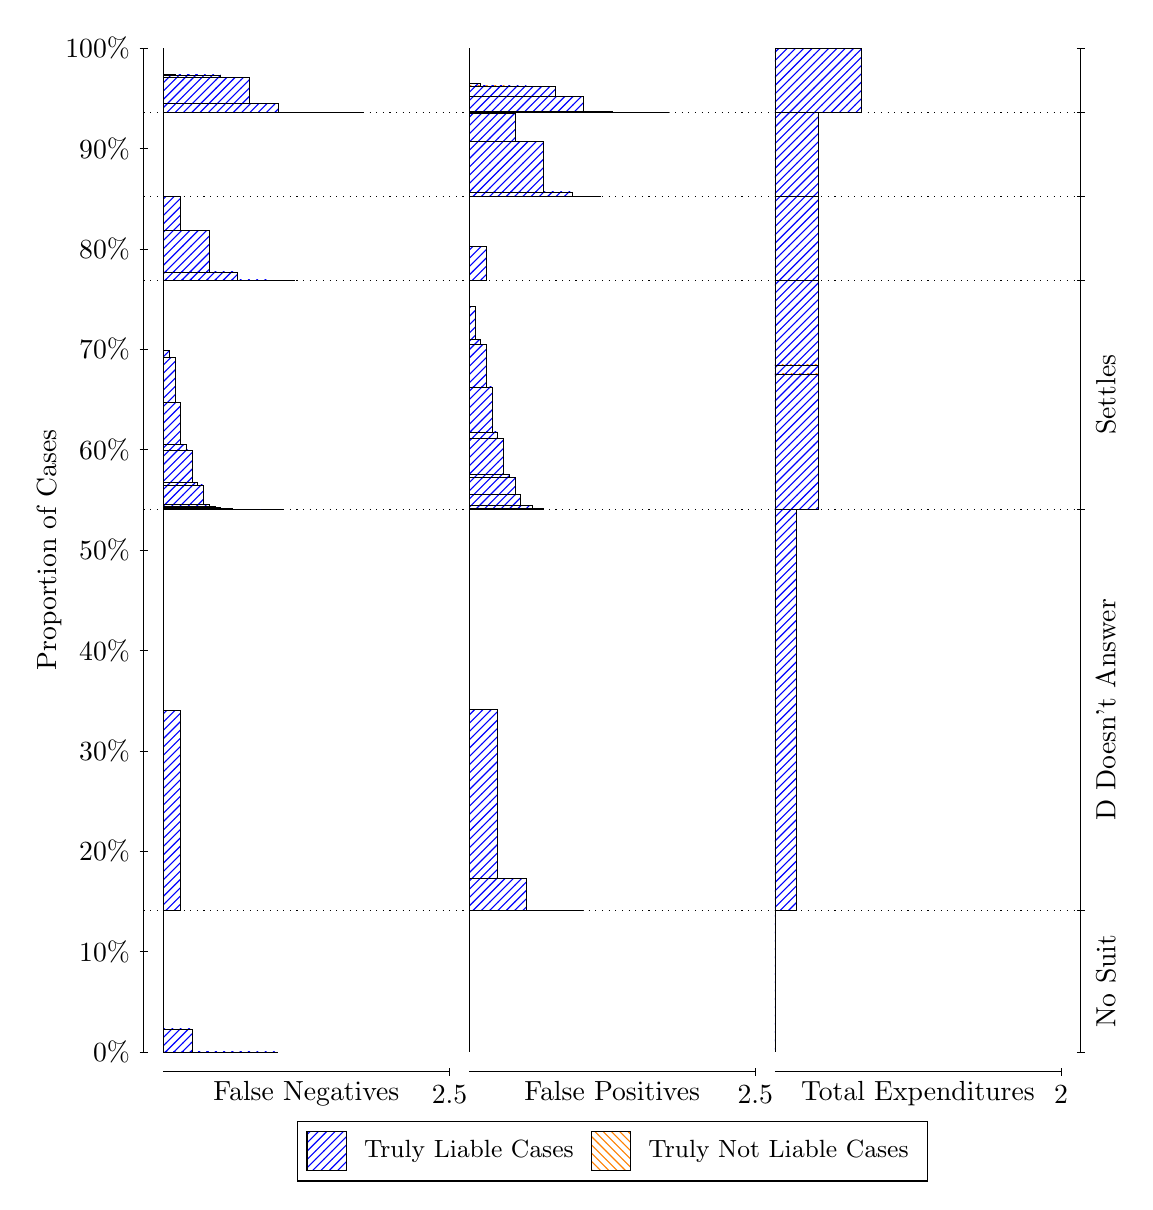
\begin{tikzpicture}
\draw[black, very thin] (1.5,1.75) -- (1.5,14.5);
\node[rotate=90, text=black, anchor=center] at (0.3, 8.125) {Proportion of Cases};
\draw[black, very thin] (1.45,1.75) -- (1.55,1.75);
\node[text=black, anchor=east] at (1.45, 1.75) {0\%};
\draw[black, very thin] (1.45,3.025) -- (1.55,3.025);
\node[text=black, anchor=east] at (1.45, 3.025) {10\%};
\draw[black, very thin] (1.45,4.3) -- (1.55,4.3);
\node[text=black, anchor=east] at (1.45, 4.3) {20\%};
\draw[black, very thin] (1.45,5.575) -- (1.55,5.575);
\node[text=black, anchor=east] at (1.45, 5.575) {30\%};
\draw[black, very thin] (1.45,6.85) -- (1.55,6.85);
\node[text=black, anchor=east] at (1.45, 6.85) {40\%};
\draw[black, very thin] (1.45,8.125) -- (1.55,8.125);
\node[text=black, anchor=east] at (1.45, 8.125) {50\%};
\draw[black, very thin] (1.45,9.4) -- (1.55,9.4);
\node[text=black, anchor=east] at (1.45, 9.4) {60\%};
\draw[black, very thin] (1.45,10.675) -- (1.55,10.675);
\node[text=black, anchor=east] at (1.45, 10.675) {70\%};
\draw[black, very thin] (1.45,11.95) -- (1.55,11.95);
\node[text=black, anchor=east] at (1.45, 11.95) {80\%};
\draw[black, very thin] (1.45,13.225) -- (1.55,13.225);
\node[text=black, anchor=east] at (1.45, 13.225) {90\%};
\draw[black, very thin] (1.45,14.5) -- (1.55,14.5);
\node[text=black, anchor=east] at (1.45, 14.5) {100\%};

\draw[black, very thin] (13.4,1.75) -- (13.4,14.5);
\draw[black, very thin] (13.35,1.75) -- (13.45,1.75);
\node[anchor=west] at (13.35, 1.75) {};
\draw[black, very thin] (13.35,3.5454) -- (13.45,3.5454);
\node[anchor=west] at (13.35, 3.5454) {};
\draw[black, very thin] (13.35,8.6433) -- (13.45,8.6433);
\node[anchor=west] at (13.35, 8.6433) {};
\draw[black, very thin] (13.35,11.552) -- (13.45,11.552);
\node[anchor=west] at (13.35, 11.552) {};
\draw[black, very thin] (13.35,12.613) -- (13.45,12.613);
\node[anchor=west] at (13.35, 12.613) {};
\draw[black, very thin] (13.35,13.678) -- (13.45,13.678);
\node[anchor=west] at (13.35, 13.678) {};
\draw[black, very thin] (13.35,14.5) -- (13.45,14.5);
\node[anchor=west] at (13.35, 14.5) {};

\draw[black, very thin, pattern color=blue, pattern=north east lines] (1.75,1.75) rectangle (3.2033,1.75);
\draw[black, very thin, pattern color=blue, pattern=north east lines] (1.75,1.75) rectangle (2.84,1.75);
\draw[black, very thin, pattern color=blue, pattern=north east lines] (1.75,1.75) rectangle (2.4767,1.7525);
\draw[black, very thin, pattern color=blue, pattern=north east lines] (1.75,1.7525) rectangle (2.1133,2.044);
\draw[black, very thin, pattern color=orange, pattern=north west lines] (1.75,2.044) rectangle (1.75,2.044);
\draw[black, very thin, pattern color=blue, pattern=north east lines] (1.75,2.044) rectangle (1.75,3.5454);
\draw[black, very thin, pattern color=blue, pattern=north east lines] (1.75,3.5454) rectangle (1.968,6.0912);
\draw[black, very thin, pattern color=orange, pattern=north west lines] (1.75,6.0912) rectangle (1.75,6.0912);
\draw[black, very thin, pattern color=blue, pattern=north east lines] (1.75,6.0912) rectangle (1.75,8.6433);
\draw[black, very thin, pattern color=blue, pattern=north east lines] (1.75,8.6433) rectangle (3.276,8.6433);
\draw[black, very thin, pattern color=blue, pattern=north east lines] (1.75,8.6433) rectangle (3.1307,8.6433);
\draw[black, very thin, pattern color=blue, pattern=north east lines] (1.75,8.6433) rectangle (2.9853,8.6433);
\draw[black, very thin, pattern color=blue, pattern=north east lines] (1.75,8.6433) rectangle (2.9127,8.6433);
\draw[black, very thin, pattern color=blue, pattern=north east lines] (1.75,8.6433) rectangle (2.84,8.6433);
\draw[black, very thin, pattern color=blue, pattern=north east lines] (1.75,8.6433) rectangle (2.7673,8.6436);
\draw[black, very thin, pattern color=blue, pattern=north east lines] (1.75,8.6436) rectangle (2.6947,8.6436);
\draw[black, very thin, pattern color=blue, pattern=north east lines] (1.75,8.6436) rectangle (2.622,8.6503);
\draw[black, very thin, pattern color=blue, pattern=north east lines] (1.75,8.6503) rectangle (2.5493,8.6511);
\draw[black, very thin, pattern color=blue, pattern=north east lines] (1.75,8.6511) rectangle (2.4767,8.6649);
\draw[black, very thin, pattern color=blue, pattern=north east lines] (1.75,8.6649) rectangle (2.404,8.6809);
\draw[black, very thin, pattern color=blue, pattern=north east lines] (1.75,8.6809) rectangle (2.3313,8.7044);
\draw[black, very thin, pattern color=blue, pattern=north east lines] (1.75,8.7044) rectangle (2.2587,8.9532);
\draw[black, very thin, pattern color=blue, pattern=north east lines] (1.75,8.9532) rectangle (2.186,8.9806);
\draw[black, very thin, pattern color=blue, pattern=north east lines] (1.75,8.9806) rectangle (2.1133,9.3964);
\draw[black, very thin, pattern color=blue, pattern=north east lines] (1.75,9.3964) rectangle (2.0407,9.4616);
\draw[black, very thin, pattern color=blue, pattern=north east lines] (1.75,9.4616) rectangle (1.968,9.9996);
\draw[black, very thin, pattern color=blue, pattern=north east lines] (1.75,9.9996) rectangle (1.8953,10.57);
\draw[black, very thin, pattern color=blue, pattern=north east lines] (1.75,10.57) rectangle (1.8227,10.656);
\draw[black, very thin, pattern color=orange, pattern=north west lines] (1.75,10.656) rectangle (1.75,10.656);
\draw[black, very thin, pattern color=blue, pattern=north east lines] (1.75,10.656) rectangle (1.75,11.552);
\draw[black, very thin, pattern color=blue, pattern=north east lines] (1.75,11.552) rectangle (3.4213,11.552);
\draw[black, very thin, pattern color=blue, pattern=north east lines] (1.75,11.552) rectangle (3.058,11.554);
\draw[black, very thin, pattern color=blue, pattern=north east lines] (1.75,11.554) rectangle (2.6947,11.658);
\draw[black, very thin, pattern color=blue, pattern=north east lines] (1.75,11.658) rectangle (2.3313,12.186);
\draw[black, very thin, pattern color=blue, pattern=north east lines] (1.75,12.186) rectangle (1.968,12.613);
\draw[black, very thin, pattern color=orange, pattern=north west lines] (1.75,12.613) rectangle (1.75,12.613);
\draw[black, very thin, pattern color=blue, pattern=north east lines] (1.75,12.613) rectangle (1.968,12.617);
\draw[black, very thin, pattern color=orange, pattern=north west lines] (1.75,12.617) rectangle (1.75,12.617);
\draw[black, very thin, pattern color=blue, pattern=north east lines] (1.75,12.617) rectangle (1.75,13.678);
\draw[black, very thin, pattern color=blue, pattern=north east lines] (1.75,13.678) rectangle (4.2933,13.678);
\draw[black, very thin, pattern color=blue, pattern=north east lines] (1.75,13.678) rectangle (3.93,13.678);
\draw[black, very thin, pattern color=blue, pattern=north east lines] (1.75,13.678) rectangle (3.5667,13.682);
\draw[black, very thin, pattern color=blue, pattern=north east lines] (1.75,13.682) rectangle (3.2033,13.793);
\draw[black, very thin, pattern color=blue, pattern=north east lines] (1.75,13.793) rectangle (2.84,14.128);
\draw[black, very thin, pattern color=blue, pattern=north east lines] (1.75,14.128) rectangle (2.622,14.128);
\draw[black, very thin, pattern color=blue, pattern=north east lines] (1.75,14.128) rectangle (2.4767,14.159);
\draw[black, very thin, pattern color=blue, pattern=north east lines] (1.75,14.159) rectangle (2.2587,14.159);
\draw[black, very thin, pattern color=blue, pattern=north east lines] (1.75,14.159) rectangle (2.2587,14.159);
\draw[black, very thin, pattern color=blue, pattern=north east lines] (1.75,14.159) rectangle (2.1133,14.16);
\draw[black, very thin, pattern color=blue, pattern=north east lines] (1.75,14.16) rectangle (1.8953,14.16);
\draw[black, very thin, pattern color=blue, pattern=north east lines] (1.75,14.16) rectangle (1.8953,14.166);
\draw[black, very thin, pattern color=orange, pattern=north west lines] (1.75,14.166) rectangle (1.75,14.166);
\draw[black, very thin, pattern color=blue, pattern=north east lines] (1.75,14.166) rectangle (1.75,14.5);
\draw[black, very thin, pattern color=orange, pattern=north west lines] (5.6333,1.75) rectangle (5.6333,1.75);
\draw[black, very thin, pattern color=blue, pattern=north east lines] (5.6333,1.75) rectangle (5.6333,3.5454);
\draw[black, very thin, pattern color=orange, pattern=north west lines] (5.6333,3.5454) rectangle (7.0867,3.5454);
\draw[black, very thin, pattern color=blue, pattern=north east lines] (5.6333,3.5454) rectangle (7.0867,3.5454);
\draw[black, very thin, pattern color=blue, pattern=north east lines] (5.6333,3.5454) rectangle (6.7233,3.5484);
\draw[black, very thin, pattern color=blue, pattern=north east lines] (5.6333,3.5484) rectangle (6.36,3.9526);
\draw[black, very thin, pattern color=blue, pattern=north east lines] (5.6333,3.9526) rectangle (5.9967,6.0975);
\draw[black, very thin, pattern color=blue, pattern=north east lines] (5.6333,6.0975) rectangle (5.6333,8.6433);
\draw[black, very thin, pattern color=orange, pattern=north west lines] (5.6333,8.6433) rectangle (6.578,8.6433);
\draw[black, very thin, pattern color=blue, pattern=north east lines] (5.6333,8.6433) rectangle (6.578,8.658);
\draw[black, very thin, pattern color=orange, pattern=north west lines] (5.6333,8.658) rectangle (6.4327,8.658);
\draw[black, very thin, pattern color=blue, pattern=north east lines] (5.6333,8.658) rectangle (6.4327,8.6934);
\draw[black, very thin, pattern color=orange, pattern=north west lines] (5.6333,8.6934) rectangle (6.2873,8.6934);
\draw[black, very thin, pattern color=blue, pattern=north east lines] (5.6333,8.6934) rectangle (6.2873,8.8267);
\draw[black, very thin, pattern color=blue, pattern=north east lines] (5.6333,8.8267) rectangle (6.2147,9.0489);
\draw[black, very thin, pattern color=orange, pattern=north west lines] (5.6333,9.0489) rectangle (6.142,9.0489);
\draw[black, very thin, pattern color=blue, pattern=north east lines] (5.6333,9.0489) rectangle (6.142,9.0836);
\draw[black, very thin, pattern color=blue, pattern=north east lines] (5.6333,9.0836) rectangle (6.0693,9.5389);
\draw[black, very thin, pattern color=orange, pattern=north west lines] (5.6333,9.5389) rectangle (5.9967,9.5389);
\draw[black, very thin, pattern color=blue, pattern=north east lines] (5.6333,9.5389) rectangle (5.9967,9.6253);
\draw[black, very thin, pattern color=blue, pattern=north east lines] (5.6333,9.6253) rectangle (5.924,10.196);
\draw[black, very thin, pattern color=blue, pattern=north east lines] (5.6333,10.196) rectangle (5.8513,10.734);
\draw[black, very thin, pattern color=blue, pattern=north east lines] (5.6333,10.734) rectangle (5.7787,10.799);
\draw[black, very thin, pattern color=blue, pattern=north east lines] (5.6333,10.799) rectangle (5.706,11.215);
\draw[black, very thin, pattern color=blue, pattern=north east lines] (5.6333,11.215) rectangle (5.6333,11.552);
\draw[black, very thin, pattern color=orange, pattern=north west lines] (5.6333,11.552) rectangle (5.8513,11.552);
\draw[black, very thin, pattern color=blue, pattern=north east lines] (5.6333,11.552) rectangle (5.8513,11.979);
\draw[black, very thin, pattern color=blue, pattern=north east lines] (5.6333,11.979) rectangle (5.6333,12.613);
\draw[black, very thin, pattern color=orange, pattern=north west lines] (5.6333,12.613) rectangle (7.3047,12.613);
\draw[black, very thin, pattern color=blue, pattern=north east lines] (5.6333,12.613) rectangle (7.3047,12.613);
\draw[black, very thin, pattern color=blue, pattern=north east lines] (5.6333,12.613) rectangle (6.9413,12.674);
\draw[black, very thin, pattern color=blue, pattern=north east lines] (5.6333,12.674) rectangle (6.578,13.318);
\draw[black, very thin, pattern color=blue, pattern=north east lines] (5.6333,13.318) rectangle (6.2147,13.673);
\draw[black, very thin, pattern color=blue, pattern=north east lines] (5.6333,13.673) rectangle (5.8513,13.678);
\draw[black, very thin, pattern color=orange, pattern=north west lines] (5.6333,13.678) rectangle (8.1767,13.678);
\draw[black, very thin, pattern color=blue, pattern=north east lines] (5.6333,13.678) rectangle (8.1767,13.678);
\draw[black, very thin, pattern color=orange, pattern=north west lines] (5.6333,13.678) rectangle (7.8133,13.678);
\draw[black, very thin, pattern color=blue, pattern=north east lines] (5.6333,13.678) rectangle (7.8133,13.678);
\draw[black, very thin, pattern color=orange, pattern=north west lines] (5.6333,13.678) rectangle (7.45,13.678);
\draw[black, very thin, pattern color=blue, pattern=north east lines] (5.6333,13.678) rectangle (7.45,13.698);
\draw[black, very thin, pattern color=orange, pattern=north west lines] (5.6333,13.698) rectangle (7.0867,13.698);
\draw[black, very thin, pattern color=blue, pattern=north east lines] (5.6333,13.698) rectangle (7.0867,13.882);
\draw[black, very thin, pattern color=blue, pattern=north east lines] (5.6333,13.882) rectangle (6.7233,14.012);
\draw[black, very thin, pattern color=blue, pattern=north east lines] (5.6333,14.012) rectangle (6.36,14.018);
\draw[black, very thin, pattern color=orange, pattern=north west lines] (5.6333,14.018) rectangle (6.142,14.018);
\draw[black, very thin, pattern color=blue, pattern=north east lines] (5.6333,14.018) rectangle (6.142,14.018);
\draw[black, very thin, pattern color=blue, pattern=north east lines] (5.6333,14.018) rectangle (5.9967,14.018);
\draw[black, very thin, pattern color=orange, pattern=north west lines] (5.6333,14.018) rectangle (5.7787,14.018);
\draw[black, very thin, pattern color=blue, pattern=north east lines] (5.6333,14.018) rectangle (5.7787,14.05);
\draw[black, very thin, pattern color=orange, pattern=north west lines] (5.6333,14.05) rectangle (5.6333,14.05);
\draw[black, very thin, pattern color=blue, pattern=north east lines] (5.6333,14.05) rectangle (5.6333,14.5);
\draw[black, very thin, pattern color=orange, pattern=north west lines] (9.5167,1.75) rectangle (9.5167,1.75);
\draw[black, very thin, pattern color=blue, pattern=north east lines] (9.5167,1.75) rectangle (9.5167,3.5454);
\draw[black, very thin, pattern color=orange, pattern=north west lines] (9.5167,3.5454) rectangle (9.7892,3.5454);
\draw[black, very thin, pattern color=blue, pattern=north east lines] (9.5167,3.5454) rectangle (9.7892,8.6433);
\draw[black, very thin, pattern color=orange, pattern=north west lines] (9.5167,8.6433) rectangle (10.062,8.6433);
\draw[black, very thin, pattern color=blue, pattern=north east lines] (9.5167,8.6433) rectangle (10.062,10.362);
\draw[black, very thin, pattern color=orange, pattern=north west lines] (9.5167,10.362) rectangle (10.062,10.362);
\draw[black, very thin, pattern color=blue, pattern=north east lines] (9.5167,10.362) rectangle (10.062,10.476);
\draw[black, very thin, pattern color=orange, pattern=north west lines] (9.5167,10.476) rectangle (10.062,10.476);
\draw[black, very thin, pattern color=blue, pattern=north east lines] (9.5167,10.476) rectangle (10.062,11.552);
\draw[black, very thin, pattern color=orange, pattern=north west lines] (9.5167,11.552) rectangle (10.062,11.552);
\draw[black, very thin, pattern color=blue, pattern=north east lines] (9.5167,11.552) rectangle (10.062,12.613);
\draw[black, very thin, pattern color=orange, pattern=north west lines] (9.5167,12.613) rectangle (10.062,12.613);
\draw[black, very thin, pattern color=blue, pattern=north east lines] (9.5167,12.613) rectangle (10.062,13.678);
\draw[black, very thin, pattern color=orange, pattern=north west lines] (9.5167,13.678) rectangle (10.607,13.678);
\draw[black, very thin, pattern color=blue, pattern=north east lines] (9.5167,13.678) rectangle (10.607,14.5);
\draw[black, dotted] (1.5,3.5454) -- (13.4,3.5454);
\draw[black, dotted] (1.5,8.6433) -- (13.4,8.6433);
\draw[black, dotted] (1.5,11.552) -- (13.4,11.552);
\draw[black, dotted] (1.5,12.613) -- (13.4,12.613);
\draw[black, dotted] (1.5,13.678) -- (13.4,13.678);
\draw[black, very thin] (1.75,1.5) -- (5.3833,1.5);
\node[text=black, anchor=north] at (3.5667, 1.5) {False Negatives};
\draw[black, very thin] (5.3833,1.45) -- (5.3833,1.55);
\node[text=black, anchor=north] at (5.3833, 1.45) {2.5};

\draw[black, very thin] (5.6333,1.5) -- (9.2667,1.5);
\node[text=black, anchor=north] at (7.45, 1.5) {False Positives};
\draw[black, very thin] (9.2667,1.45) -- (9.2667,1.55);
\node[text=black, anchor=north] at (9.2667, 1.45) {2.5};

\draw[black, very thin] (9.5167,1.5) -- (13.15,1.5);
\node[text=black, anchor=north] at (11.333, 1.5) {Total Expenditures};
\draw[black, very thin] (13.15,1.45) -- (13.15,1.55);
\node[text=black, anchor=north] at (13.15, 1.45) {2};

\node[text=black, centered, rotate=90] at (13.72, 2.6477) {No Suit};
\node[text=black, centered, rotate=90] at (13.72, 6.0943) {D Doesn't Answer};
\node[text=black, centered, rotate=90] at (13.72, 10.098) {Settles};




\draw (7.449999999999999,1.5) node[draw=none] (baseCoordinate) {};
\begin{scope}[align=center]
        \matrix[scale=0.5, draw=black, below=0.5cm of baseCoordinate, nodes={draw}, column sep=0.1cm]{
            \node[rectangle, draw, minimum width=0.5cm, minimum height=0.5cm, pattern color=blue, pattern=north east lines] {}; &
            \node[draw=none, font=\small, text=black] (B) {Truly Liable Cases}; &
            \node[rectangle, draw, minimum width=0.5cm, minimum height=0.5cm, pattern color=orange, pattern=north west lines] {}; &
            \node[draw=none, font=\small, text=black] (B) {Truly Not Liable Cases}; \\
            };
\end{scope}

\end{tikzpicture}
\end{document}